\documentclass[aspectratio=169]{beamer}

\usepackage{xcolor}
\usepackage{mathtools}
\usepackage{amsfonts}
\usepackage{bm}

\usetheme{default}
\usefonttheme{serif}

\definecolor{dpasp-orange}{HTML}{ff3a20}
\definecolor{dpasp-green}{HTML}{5b8c5a}
\definecolor{dpasp-blue}{HTML}{0e79b2}
\definecolor{dpasp-yellow}{HTML}{f5b700}
\definecolor{dpasp-dgreen}{HTML}{1e2f23}
\definecolor{dpasp-purple}{HTML}{331832}
\definecolor{dark gray}{HTML}{808080}
\definecolor{darker gray}{HTML}{606060}

\definecolor{palette1}{HTML}{003049}
\definecolor{palette2}{HTML}{a62639}
\definecolor{palette3}{HTML}{f77f00}
\definecolor{palette4}{HTML}{3bb273}
\definecolor{palette5}{HTML}{4d9de0}
\definecolor{palette6}{HTML}{d7cf07}
\definecolor{palette7}{HTML}{97b1a6}
\definecolor{palette8}{HTML}{386641}

\usepackage{times}
\usepackage{soul}
\usepackage{inconsolata}
\usepackage{minted}
\definecolor{mintedframe}{HTML}{5ca4a9}
\setminted{
    fontsize=\small,
    escapeinside=&&,
    rulecolor=mintedframe,
}
\usemintedstyle{sas}
\newminted[pasp]{pasp}{mathescape}
\newmintinline[paspi]{pasp}{mathescape,fontsize=\huge}
\newmintinline[paspin]{pasp}{mathescape,fontsize=\normalsize}
\newmintedfile[paspf]{pasp}{mathescape}

\usepackage{tikz}
\usetikzlibrary{shapes}
\usetikzlibrary{shapes.multipart}
\usetikzlibrary{fit}
\usetikzlibrary{decorations.pathreplacing,calligraphy,calc}
\usetikzlibrary{arrows.meta,matrix,arrows}

\newcommand\blfootnote[1]{%
  \begingroup
  \renewcommand\thefootnote{}\footnote{#1}%
  \addtocounter{footnote}{-1}%
  \endgroup
}

\newcommand{\dpasp}{\textbf{\textcolor{dpasp-purple}{$\bm{d}$}\,\textcolor{dpasp-orange}{$\pmb{\mathbb{P}}$}\textcolor{dpasp-green}{A}\textcolor{dpasp-blue}{S}\textcolor{dpasp-yellow}{P}}}
\newcommand{\dpaspnc}{\textbf{$\bm{d}$\,$\pmb{\mathbb{P}}$ASP}}

\usepackage{pgfplots}
\pgfplotsset{compat=1.18}

%\author{\small\textbf{Renato Lui Geh}, Jonas Gonçalves, Igor Cataneo Silveira,\texorpdfstring{\\}{ }Denis Deratani Mauá, Fabio Gagliardi Cozman}
%\subtitle{\texorpdfstring{\normalsize\color{darker gray}\itshape}{}\textcolor{dpasp-blue}{D}ifferentiable \textcolor{dpasp-blue}{P}robabilistic \textcolor{dpasp-blue}{A}nswer \textcolor{dpasp-blue}{S}et \textcolor{dpasp-blue}{P}rogramming\\For Neurosymbolic Learning and Reasoning}
\date{}
%\institute{\small\textbf{University of São Paulo}}

\makeatletter
\setbeamertemplate{title page}[default][left]
\makeatother

\begin{document}

\title{\rmfamily\Huge\color{black}An Online Interpreter for\\\quad\textbf{\textcolor{dpasp-purple}{$\bm{d}$}\,\textcolor{dpasp-orange}{$\pmb{\mathbb{P}}$}\textcolor{dpasp-green}{A}\textcolor{dpasp-blue}{S}\textcolor{dpasp-yellow}{P}}}

\begin{frame}
%    \begin{tikzpicture}[remember picture,overlay]
%        \node[anchor=north east] at (current page.north east) {\includegraphics[width=0.4\textwidth]{imgs/campus.png}};
%    \end{tikzpicture}
  \rmfamily\LARGE\color{black}An Online Interpreter for

  \vspace{0.25cm}

  \begin{center}
    \Huge
    \textbf{\textcolor{dpasp-purple}{$\bm{d}$}\,\textcolor{dpasp-orange}{$\pmb{\mathbb{P}}$}\textcolor{dpasp-green}{A}\textcolor{dpasp-blue}{S}\textcolor{dpasp-yellow}{P}}
  \end{center}

  \vfill

  \normalsize
  \textcolor{darker gray}{\textcolor{dpasp-blue}{D}ifferentiable
    \textcolor{dpasp-blue}{P}robabilistic \textcolor{dpasp-blue}{A}nswer
    \textcolor{dpasp-blue}{S}et \textcolor{dpasp-blue}{P}rogramming\\For Neurosymbolic Learning and
    Reasoning}

  \vfill

  \small Renato Lui Geh\textcolor{dark gray}{, Jonas Gonçalves, Igor Cataneo Silveira,\\Denis
    Deratani Mauá, Fabio Gagliardi Cozman}
\end{frame}

\setbeamercolor{frametitle}{bg=dpasp-yellow,fg=white}
\begin{frame}{\textbf{$\bm{d}\,\pmb{\mathbb{P}}$ASP for Neurosymbolic Learning and Reasoning}}
\centering
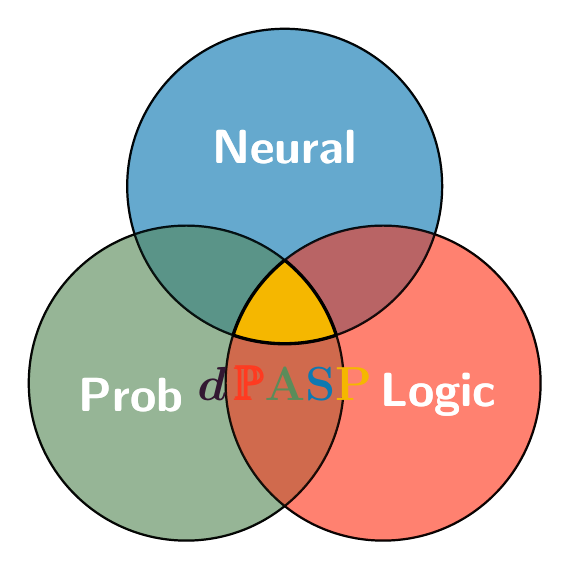
\begin{tikzpicture}
    \onslide<1>{
        \node (neural) at (0, 1.25) {};
        \node (prob) at (-1.25, -1.25) {};
        \node (logic) at (1.25, -1.25) {};
        \fill[dpasp-blue,opacity=0.6] (neural) circle (2);
        \fill[dpasp-green,opacity=0.6] (prob) circle (2);
        \fill[dpasp-orange,opacity=0.6] (logic) circle (2);
        \draw[thick] (neural) circle (2) node[yshift=0.5cm,opacity=1.0] {\sf\LARGE\color{white}\textbf{Neural}};
        \draw[thick] (prob) circle (2) node[xshift=-0.7cm,yshift=-0.15cm,opacity=1.0] {\sf\LARGE\color{white}\textbf{Prob}};
        \draw[thick] (logic) circle (2) node[xshift=0.7cm,yshift=-0.15cm,opacity=1.0] {\sf\LARGE\color{white}\textbf{Logic}};
    }
    \onslide<2->{
        \node (neural) at (0, 1.25) {};
        \node (prob) at (-1.25, -1.25) {};
        \node (logic) at (1.25, -1.25) {};
        \fill[dpasp-blue,opacity=0.1] (neural) circle (2);
        \fill[dpasp-green,opacity=0.1] (prob) circle (2);
        \fill[dpasp-orange,opacity=0.1] (logic) circle (2);
        \draw[opacity=0.1,thick] (neural) circle (2) node[yshift=0.5cm,opacity=1.0] {\sf\LARGE\color{white}\textbf{Neural}};
        \draw[opacity=0.1,thick] (prob) circle (2) node[xshift=-0.7cm,yshift=-0.15cm,opacity=1.0] {\sf\LARGE\color{white}\textbf{Prob}};
        \draw[opacity=0.1,thick] (logic) circle (2) node[xshift=0.7cm,yshift=-0.15cm,opacity=1.0] {\sf\LARGE\color{white}\textbf{Logic}};
        \scope
        \clip (neural) circle (2);
        \clip (logic) circle (2);
        \fill[dpasp-yellow] (prob) circle (2);
        \draw[very thick] (prob) circle (2);
        \endscope
        \scope
        \clip (prob) circle (2);
        \clip (logic) circle (2);
        \draw[very thick] (neural) circle (2);
        \endscope
        \scope
        \clip (prob) circle (2);
        \clip (neural) circle (2);
        \draw[very thick] (logic) circle (2);
        \endscope
        \node[yshift=-1.25cm] at (0, 0) {\LARGE\textbf{\textcolor{dpasp-purple}{$\bm{d}$}\,\textcolor{dpasp-orange}{$\pmb{\mathbb{P}}$}\textcolor{dpasp-green}{A}\textcolor{dpasp-blue}{S}\textcolor{dpasp-yellow}{P}}};
    }
\end{tikzpicture}
\end{frame}

\newcommand{\inlineimg}[1]{\raisebox{-.25\height}{\includegraphics[height=1em]{imgs/#1}}}

\setbeamercolor{frametitle}{bg=dpasp-blue,fg=white}
\begin{frame}[fragile]{\textbf{Language}}

\vspace{0.5cm}

\textbf{\underline{\color{dpasp-green}Example:}} Parsing arithmetic expressions, e.g.\ \paspin{X + Y} $=f($\inlineimg{8_0}$)+f($\inlineimg{3_0}$)=\,?$

\vspace{0.5cm}

\begin{pasp}
% neural rule
?::digit(Image, {0..9}) :- data(Image).
% data loaders -- interact with Python code
data(img1) &$\sim$& test(@mnist_test), train(@mnist_train).
data(img2) &$\sim$& test(@mnist_test), train(@mnist_train).
% prob. answer set program
add(Z) :- digit(I, X), digit(J, Y), Z = X + Y.
subtract(Z) :- digit(I, X), digit(J, Y), Z = X - Y.
multiply(Z) :- digit(I, X), digit(J, Y), Z = X * Y.
% learn the program end-to-end and pass learning parameters
#learn @mnist_sum, lr = 1., niters = 5, ..., batch = 1000.
% inference: what is the probability of X + Y = 14 given X = 8?
#query add(11) | digit(img1, 8).
\end{pasp}
\scalebox{0.5}{
\begin{tikzpicture}[remember picture,overlay]
    \tikzstyle{neuron}=[circle,draw,color=dark gray,minimum size=0.5cm,ultra thick,inner sep=0pt]
    \tikzset{nedge/.style={color=dark gray,ultra thick}}
    \node (origin) at ($(current page.north east) + (6, -0.75)$) {};
    \node[inner sep=0pt,label={[xshift=-0.5cm]north:\tiny\paspi{img1}}] (input1) at ($(origin) + (0, 1.0)$) {\includegraphics[height=1cm]{imgs/8_0.png}};
    \node[inner sep=0pt,label={[xshift=-0.5cm]south:\tiny\paspi{img2}}] (input2) at ($(origin) + (0, -1.0)$) {\includegraphics[height=1cm]{imgs/3_0.png}};
    \foreach \i in {-2,...,2} {
        \node[neuron] (f\i) at ($(origin) + (2.0, 2*\i)$) {};
        \draw[nedge] (input1) -- (f\i);
        \draw[nedge] (input2) -- (f\i);
    }
    \foreach \i in {-2,...,2} {
        \node[neuron] (g\i) at ($(f\i) + (2.0, 0)$) {};
    }
    \foreach \i in {-2,...,2} {
        \foreach \j in {-2,...,2} {
            \draw[nedge] (f\i) -- (g\j);
        }
    }
    \node[rotate=90] (p0) at ($(g0) + (2, 0)$) {\color{dark gray}\footnotesize$\bm{\cdots}$};
    \node[neuron,label=east:\tiny\paspi{f(0)}] (p-2) at ($(g-2) + (2, 0)$) {};
    \node[neuron,label=east:\tiny\paspi{f(1)}] (p-1) at ($(g-1) + (2, 0)$) {};
    \node[neuron,label=east:\tiny\paspi{f(8)}] (p1) at ($(g1) + (2, 0)$) {};
    \node[neuron,label=east:\tiny\paspi{f(9)}] (p2) at ($(g2) + (2, 0)$) {};
    \foreach \i in {-2,...,2} {
        \foreach \j in {-2,...,2} {
            \ifthenelse{\j=0}{}{\draw[nedge] (g\i) -- (p\j.west);}
        }
    }
\end{tikzpicture}
}
\end{frame}

\setbeamercolor{frametitle}{bg=dpasp-green,fg=white}
\begin{frame}[fragile]{\textbf{Semantics}}
\resizebox{\textwidth}{!}{
\begin{tikzpicture}
    \tikzstyle{neuron}=[circle,draw,color=dark gray,minimum size=0.5cm,ultra thick,inner sep=0pt]
    \tikzset{nedge/.style={color=dark gray,ultra thick}}
    \node[inner sep=0pt,label={[xshift=-0.5cm]north:\Huge\paspi{img1}}] (input1) at (0, 1.0) {\includegraphics[height=1cm]{imgs/8_0.png}};
    \node[inner sep=0pt,label={[xshift=-0.5cm]south:\Huge\paspi{img2}}] (input2) at (0, -1.0) {\includegraphics[height=1cm]{imgs/3_0.png}};
    \foreach \i in {-2,...,2} {
        \node[neuron] (f\i) at (2.0, 2*\i) {};
        \draw[nedge] (input1) -- (f\i);
        \draw[nedge] (input2) -- (f\i);
    }
    \foreach \i in {-2,...,2} {
        \node[neuron] (g\i) at ($(f\i) + (2.0, 0)$) {};
    }
    \foreach \i in {-2,...,2} {
        \foreach \j in {-2,...,2} {
            \draw[nedge] (f\i) -- (g\j);
        }
    }
    \node[rotate=90] (p0) at ($(g0) + (2, 0)$) {\color{dark gray}\footnotesize$\cdots$};
    \node[neuron,label=east:\LARGE\paspi{f(0)}] (p-2) at ($(g-2) + (2, 0)$) {};
    \node[neuron,label=east:\LARGE\paspi{f(1)}] (p-1) at ($(g-1) + (2, 0)$) {};
    \node[neuron,label=east:\LARGE\paspi{f(8)}] (p1) at ($(g1) + (2, 0)$) {};
    \node[neuron,label=east:\LARGE\paspi{f(9)}] (p2) at ($(g2) + (2, 0)$) {};
    \foreach \i in {-2,...,2} {
        \foreach \j in {-2,...,2} {
            \ifthenelse{\j=0}{}{\draw[nedge] (g\i) -- (p\j.west);}
        }
    }
    \draw (-2, 5) rectangle (9, -5);
    \node at (3.5, 5.5) {\LARGE\textsc{Neural Network}};
    \node[align=left,anchor=west,scale=0.75] at ($(-2, -5) + (0, -2)$) {\LARGE\paspi{add(Z) :- digit(I, X), digit(J, Y), ...}};
    \node[align=left,anchor=west,scale=0.75] at ($(-2, -5) + (0, -3)$) {\LARGE\paspi{subtract(Z) :- digit(I, X), digit(J,...}};
    \node[align=left,anchor=west,scale=0.75] at ($(-2, -5) + (0, -4)$) {\LARGE\paspi{multiply(Z) :- digit(I, X), digit(J,...}};
    \draw (-2, -6) rectangle (9, -10);
    \node at (3.5, -10.5) {\LARGE\textsc{Program}};

    \node (linf) at (19.5, -2) {};
    \draw (linf) rectangle ($(linf) + (9, -8)$);
    \node at ($(linf) + (4.75, -8.5)$) {\LARGE\textsc{Logic Inference}};
    \node (add) at ($(linf) + (4, -1)$) {\LARGE\paspi{add(14)}};
    \node (digit1) at ($(add) + (3, -2)$) {\LARGE\paspi{digit(8)}};
    \node (digit2) at ($(add) + (-2, -3)$) {\LARGE\paspi{digit(3)}};
    \node (sub) at ($(linf) + (2.75, -7.25)$) {\LARGE\paspi{subtract(5)}};
    \draw[->] (digit1) -- (add);
    \draw[->] (digit2) -- (add);
    \draw[->] (digit1) -- (sub);
    \draw[->] (digit2) -- (sub);

    % Neural -> prob inf
    \draw[-{Latex[length=5mm,width=4mm]}] (9, 3.5) -- (10.5, 3.5);
    \draw[color=dpasp-orange,-{Latex[length=5mm,width=4mm]}] (10.5, 1.5) -- (9, 1.5);
    % Program -> translation
    \draw[-{Latex[length=5mm,width=4mm]}] (9, -8) -- (10.5, -8);

    \node (pinf) at (10.5, 5) {};
    \draw (pinf) rectangle ($(pinf) + (13.25, -5)$);
    \node at ($(pinf) + (6.75, 0.5)$) {\LARGE\textsc{Probabilistic Inference}};
    \node[draw,shape=rectangle,dashed,color=darker gray,ultra thick,inner sep=0.75cm,minimum width=5cm,minimum height=2.5cm] at ($(pinf) + (3.25, -2.5)$) {\LARGE\color{black}\textsc{Credal}};
    \node[draw,shape=rectangle,dashed,color=darker gray,ultra thick,inner sep=0.75cm,minimum width=5cm,minimum height=2.5cm] at ($(pinf) + (9.5, -2.5)$) {\LARGE\color{black}\textsc{Max-Ent}};

    % Logic inf -> prob inf
    \draw[-{Latex[length=5mm,width=4mm]}] ($(pinf) + (11.5, -7)$) -- ($(pinf) + (11.5, -5)$);

    \node (trl) at (10.5, -2) {};
    \draw (trl) rectangle ($(trl) + (7, -8)$);
    % Translation -> logic inf
    \draw[-{Latex[length=5mm,width=4mm]}] ($(trl) + (7, -4)$) -- ($(linf) + (0, -4)$);
    \node[dashed,shape=rectangle,draw,color=darker gray,ultra thick,inner sep=0.15cm,minimum width=6.5cm,minimum height=1.5cm] (stable) at ($(trl) + (3.5, -1.25)$) {\LARGE\color{black}\textsc{Stable}};
    \node[dashed,shape=rectangle,draw,color=darker gray,ultra thick,inner sep=0.15cm,minimum width=6.5cm,minimum height=1.5cm] (partial) at ($(stable) + (0, -1.85)$) {\LARGE\color{black}\textsc{Partial}};
    \node[dashed,shape=rectangle,draw,color=darker gray,ultra thick,inner sep=0.15cm,minimum width=6.5cm,minimum height=1.5cm] (lstable) at ($(partial) + (0, -1.85)$) {\LARGE\color{black}\textsc{L-stable}};
    \node[dashed,shape=rectangle,draw,color=darker gray,ultra thick,inner sep=0.15cm,minimum width=6.5cm,minimum height=1.5cm] (smproblog) at ($(lstable) + (0, -1.85)$) {\LARGE\color{black}\textsc{SMProbLog}};
    \node at ($(trl) + (3.75, -8.5)$) {\LARGE\textsc{Translation}};

    % Prob inf -> output
    \draw[-{Latex[length=5mm,width=4mm]}] ($(pinf) + (13.25, -1.0)$) -- ($(pinf) + (15, -1.0)$);
    \draw[color=dpasp-orange,-{Latex[length=5mm,width=4mm]}]  ($(pinf) + (15, -3.0)$) -- ($(pinf) + (13.25, -3.0)$);
    \node[anchor=west,label=above:\LARGE\textsc{Output},shape=rectangle,draw,minimum width=8cm] (out) at ($(pinf) + (15,-1.0)$) {\LARGE $\mathbb{P}(\textup{query})=0.97$};
    \node[anchor=west,label=below:\LARGE\textsc{Ground-truth},shape=rectangle,draw,minimum width=8cm] (gt) at ($(pinf) + (15,-3.0)$) {\paspi{add(11)}};

    \draw[-{Latex[length=5mm,width=4mm]},ultra thick] ($(linf) + (10, -2)$) -- ($(linf) + (14, -2)$) node[pos=0.5,below=0.25cm] {\LARGE Inference flow};
    \draw[color=dpasp-orange,-{Latex[length=5mm,width=4mm]},ultra thick] ($(linf) + (14, -5)$) -- ($(linf) + (10, -5)$) node[pos=0.5,below=0.25cm] {\LARGE Update flow};
\end{tikzpicture}
}
\end{frame}

\setbeamercolor{frametitle}{bg=dpasp-orange,fg=white}
\begin{frame}[fragile]{\textbf{An Online Editor and Interpreter for \dpaspnc}}
\resizebox{\textwidth}{!}{
\begin{tikzpicture}
    \tikzstyle{neuron}=[circle,draw,color=dark gray,minimum size=0.5cm,ultra thick,inner sep=0pt]
    \tikzset{nedge/.style={color=dark gray,ultra thick}}

    \node[inner sep=0pt,label={[xshift=-0.5cm]north:\Huge\paspi{img1}}] (input1) at (0, 1.0) {\includegraphics[height=1cm]{imgs/8_0.png}};
    \node[inner sep=0pt,label={[xshift=-0.5cm]south:\Huge\paspi{img2}}] (input2) at (0, -1.0) {\includegraphics[height=1cm]{imgs/3_0.png}};
    \foreach \i in {-2,...,2} {
        \node[neuron] (f\i) at (2.0, 2*\i) {};
        \draw[nedge] (input1) -- (f\i);
        \draw[nedge] (input2) -- (f\i);
    }
    \foreach \i in {-2,...,2} {
        \node[neuron] (g\i) at ($(f\i) + (2.0, 0)$) {};
    }
    \foreach \i in {-2,...,2} {
        \foreach \j in {-2,...,2} {
            \draw[nedge] (f\i) -- (g\j);
        }
    }
    \node[rotate=90] (p0) at ($(g0) + (2, 0)$) {\color{dark gray}\footnotesize$\cdots$};
    \node[neuron,label=east:\LARGE\paspi{f(0)}] (p-2) at ($(g-2) + (2, 0)$) {};
    \node[neuron,label=east:\LARGE\paspi{f(1)}] (p-1) at ($(g-1) + (2, 0)$) {};
    \node[neuron,label=east:\LARGE\paspi{f(8)}] (p1) at ($(g1) + (2, 0)$) {};
    \node[neuron,label=east:\LARGE\paspi{f(9)}] (p2) at ($(g2) + (2, 0)$) {};
    \foreach \i in {-2,...,2} {
        \foreach \j in {-2,...,2} {
            \ifthenelse{\j=0}{}{\draw[nedge] (g\i) -- (p\j.west);}
        }
    }
    \draw (-2, 5) rectangle (9, -5);
    \node at (3.5, 5.5) {\LARGE\textsc{Neural Network}};
    \node[align=left,anchor=west,scale=0.75] at ($(-2, -5) + (0, -2)$) {\LARGE\paspi{add(Z) :- digit(I, X), digit(J, Y), ...}};
    \node[align=left,anchor=west,scale=0.75] at ($(-2, -5) + (0, -3)$) {\LARGE\paspi{subtract(Z) :- digit(I, X), digit(J,...}};
    \node[align=left,anchor=west,scale=0.75] at ($(-2, -5) + (0, -4)$) {\LARGE\paspi{multiply(Z) :- digit(I, X), digit(J,...}};
    \draw (-2, -6) rectangle (9, -10);
    \node at (3.5, -10.5) {\LARGE\textsc{Program}};

    \node (linf) at (19.5, -2) {};
    \draw (linf) rectangle ($(linf) + (9, -8)$);
    \node at ($(linf) + (4.75, -8.5)$) {\LARGE\textsc{Logic Inference}};
    \node (add) at ($(linf) + (4, -1)$) {\LARGE\paspi{add(14)}};
    \node (digit1) at ($(add) + (3, -2)$) {\LARGE\paspi{digit(8)}};
    \node (digit2) at ($(add) + (-2, -3)$) {\LARGE\paspi{digit(3)}};
    \node (sub) at ($(linf) + (2.75, -7.25)$) {\LARGE\paspi{subtract(5)}};
    \draw[->] (digit1) -- (add);
    \draw[->] (digit2) -- (add);
    \draw[->] (digit1) -- (sub);
    \draw[->] (digit2) -- (sub);

    % Neural -> prob inf
    \draw[-{Latex[length=5mm,width=4mm]}] (9, 3.5) -- (10.5, 3.5);
    \draw[color=dpasp-orange,-{Latex[length=5mm,width=4mm]}] (10.5, 1.5) -- (9, 1.5);
    % Program -> translation
    \draw[-{Latex[length=5mm,width=4mm]}] (9, -8) -- (10.5, -8);

    \node (pinf) at (10.5, 5) {};
    \draw (pinf) rectangle ($(pinf) + (13.25, -5)$);
    \node at ($(pinf) + (6.75, 0.5)$) {\LARGE\textsc{Probabilistic Inference}};
    \node[draw,shape=rectangle,dashed,color=darker gray,ultra thick,inner sep=0.75cm,minimum width=5cm,minimum height=2.5cm] at ($(pinf) + (3.25, -2.5)$) {\LARGE\color{black}\textsc{Credal}};
    \node[draw,shape=rectangle,dashed,color=darker gray,ultra thick,inner sep=0.75cm,minimum width=5cm,minimum height=2.5cm] at ($(pinf) + (9.5, -2.5)$) {\LARGE\color{black}\textsc{Max-Ent}};

    % Logic inf -> prob inf
    \draw[-{Latex[length=5mm,width=4mm]}] ($(pinf) + (11.5, -7)$) -- ($(pinf) + (11.5, -5)$);

    \node (trl) at (10.5, -2) {};
    \draw (trl) rectangle ($(trl) + (7, -8)$);
    % Translation -> logic inf
    \draw[-{Latex[length=5mm,width=4mm]}] ($(trl) + (7, -4)$) -- ($(linf) + (0, -4)$);
    \node[dashed,shape=rectangle,draw,color=darker gray,ultra thick,inner sep=0.15cm,minimum width=6.5cm,minimum height=1.5cm] (stable) at ($(trl) + (3.5, -1.25)$) {\LARGE\color{black}\textsc{Stable}};
    \node[dashed,shape=rectangle,draw,color=darker gray,ultra thick,inner sep=0.15cm,minimum width=6.5cm,minimum height=1.5cm] (partial) at ($(stable) + (0, -1.85)$) {\LARGE\color{black}\textsc{Partial}};
    \node[dashed,shape=rectangle,draw,color=darker gray,ultra thick,inner sep=0.15cm,minimum width=6.5cm,minimum height=1.5cm] (lstable) at ($(partial) + (0, -1.85)$) {\LARGE\color{black}\textsc{L-stable}};
    \node[dashed,shape=rectangle,draw,color=darker gray,ultra thick,inner sep=0.15cm,minimum width=6.5cm,minimum height=1.5cm] (smproblog) at ($(lstable) + (0, -1.85)$) {\LARGE\color{black}\textsc{SMProbLog}};
    \node at ($(trl) + (3.75, -8.5)$) {\LARGE\textsc{Translation}};

    % Prob inf -> output
    \draw[-{Latex[length=5mm,width=4mm]}] ($(pinf) + (13.25, -1.0)$) -- ($(pinf) + (15, -1.0)$);
    \draw[color=dpasp-orange,-{Latex[length=5mm,width=4mm]}]  ($(pinf) + (15, -3.0)$) -- ($(pinf) + (13.25, -3.0)$);
    \node[anchor=west,label=above:\LARGE\textsc{Output},shape=rectangle,draw,minimum width=8cm] (out) at ($(pinf) + (15,-1.0)$) {\LARGE $\mathbb{P}(\textup{query})=0.97$};
    \node[anchor=west,label=below:\LARGE\textsc{Ground-truth},shape=rectangle,draw,minimum width=8cm] (gt) at ($(pinf) + (15,-3.0)$) {\paspi{add(11)}};

    \draw[-{Latex[length=5mm,width=4mm]},ultra thick] ($(linf) + (10, -2)$) -- ($(linf) + (14, -2)$) node[pos=0.5,below=0.25cm] {\LARGE Inference flow};
    \draw[color=dpasp-orange,-{Latex[length=5mm,width=4mm]},ultra thick] ($(linf) + (14, -5)$) -- ($(linf) + (10, -5)$) node[pos=0.5,below=0.25cm] {\LARGE Update flow};

    \node (rect-south-east) at ($(linf.south east) + (15, -9)$) {};
    \draw[ultra thick] (-3, 6) rectangle (rect-south-east);
    \path (-3, 6.5) -- (rect-south-east |- 3, 6.5) node[midway] (dpasp-label) {\Huge\dpasp};

    \node[anchor=north west] (editor) at (-30, 4) {
      \begin{minipage}{\textwidth}
        \inputminted[fontsize=\huge]{pasp}{p.plp}
      \end{minipage}
    };
    \draw[ultra thick] let \p1 = ($(linf.south east) + (15, -9)$) in
      ($(editor.north west) + (-1, 2)$) rectangle (-6, \y1) node (editor-south-east) {};
    \path ($(editor.north west) + (-1, 2)$) -- (editor-south-east |- 0, 7) node[midway]
      (editor-label) {\Huge\textsc{Editor}};

    \path ($(editor.north west) + (-1, 2)$) -- (editor-south-east -| 0, 7) node[midway]
      (editor-out) {};
    \node (rect-north-west) at (-3, 6.5) {};
    \path (rect-north-west |- 5, 0) -- (rect-south-east) node[pos=0.5] (dpasp-in) {};
    \draw[line width=4pt,->,>=latex'] ($(editor-out -| -3, 0) + (-3, 0)$) -- (editor-out -| -3, 0);
    \node[inner sep=0pt] (dpasp-out) at (3, 0 |- rect-south-east) {};

    \draw[line width=4pt,->,>=latex'] (dpasp-out) -- ($(dpasp-out) + (0, -3)$);
    \node (output-in) at ($(dpasp-out) + (0, -3)$) {};
    \draw[ultra thick] ($(output-in) + (-10, 0)$) rectangle ($(output-in) + (10, -10)$);
    \node at ($(output-in) + (0, -10.5)$) {\Huge\textsc{Output}};
    \node[anchor=south] at ($(dpasp-out) + (0, -12.5)$) {
      \begin{minipage}{\textwidth}
        \begin{center}
          \paspi{&$\mathbb{P}($&add(11)&$|$&digit(img1, 8)&$)=0.3539$&}

          \vspace{0.5cm}

          \begin{tikzpicture}
            \begin{axis}[ybar,width=\textwidth,height=0.9\textheight]
              \addplot table {dpasp_out.txt};
            \end{axis}
          \end{tikzpicture}
        \end{center}
      \end{minipage}
    };
\end{tikzpicture}
}
\end{frame}

\begin{frame}
  \rmfamily\LARGE\color{black}An Online Interpreter for

  \vspace{0.25cm}

  \begin{center}
    \Huge
    \textbf{\textcolor{dpasp-purple}{$\bm{d}$}\,\textcolor{dpasp-orange}{$\pmb{\mathbb{P}}$}\textcolor{dpasp-green}{A}\textcolor{dpasp-blue}{S}\textcolor{dpasp-yellow}{P}}
  \end{center}

  \vfill

  \normalsize
  \textcolor{darker gray}{\textcolor{dpasp-blue}{D}ifferentiable
    \textcolor{dpasp-blue}{P}robabilistic \textcolor{dpasp-blue}{A}nswer
    \textcolor{dpasp-blue}{S}et \textcolor{dpasp-blue}{P}rogramming\\For Neurosymbolic Learning and
    Reasoning}

  \vfill

  \small Renato Lui Geh\textcolor{dark gray}{, Jonas Gonçalves, Igor Cataneo Silveira,\\Denis
    Deratani Mauá, Fabio Gagliardi Cozman}
\end{frame}

\end{document}
